\subsection{Peer Discovery}
\label{sec:p2p:peer-discovery}

Newly connected nodes are lacking information about existing nodes in the network and thus need the help of others to introduce them to the rest of the network. This is done using a smart contract which acts as a Schelling point holding a list of entry nodes.

Once a node intends to join the network, it first fetches


it first establishes a connection with the entry nodes and receives information about other nodes in the network.

To get the most recent announcements as well as past ones, nodes either need to run their own Ethereum node or connect to a Web3 provider.

creates a secondary channel and

to which new nodes can connect to and learn about other nodes in the network. At startup, nodes need either run their own Ethereum node a or connect to a Web3 provider to fetch a list of nodes that have announced themselves as entry nodes.

In addition, each node announces itself within the smart contract such that other nodes can about the existence the newly connected node. This step is necessary for all nodes because all nodes nodes need to maintain a mapping between Ethereum addresses and public key in order to construct mixnet packets, see section \ref{sec:sphinx}, and to handle incentives for relaying packets, see \ref{sec:incentives}. HOPR thereby destinguishes two types of announcements: routable addresses of nodes who act as entry nodes and non-routable addresses that solely contain the nodes' public key.

\begin{figure}[H]
    \centering

    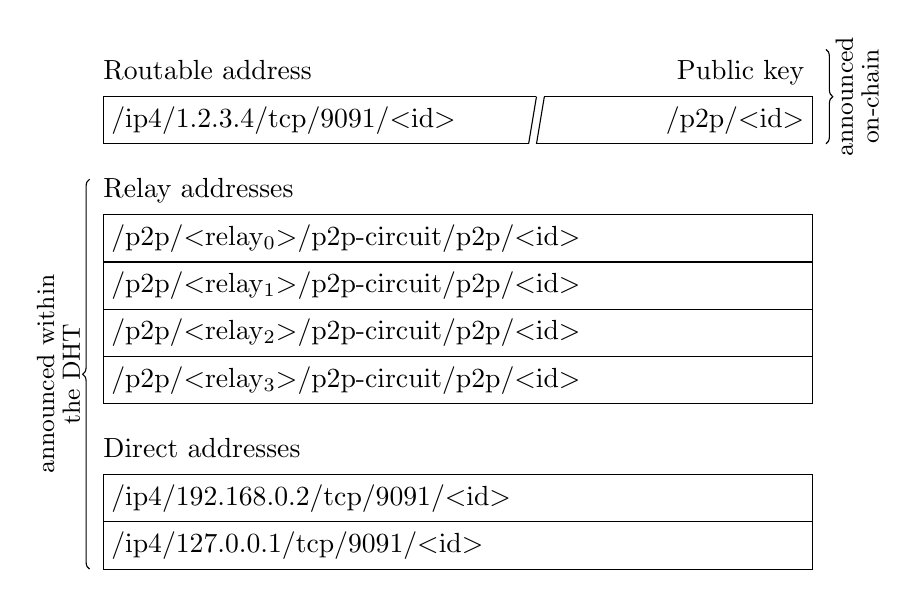
\begin{tikzpicture}
        \def\one{0.6}
        \def\nodeWidth{9}
        \def\nodeWidthMinusPadding{8.8}
        \def\nodeHeight{\one}
        \def\padding{0.1}
        \def\numberOfRelays{3} % +1
        \def\nodeOffset{1}

        % Routable address
        \path (0,0) rectangle (\nodeWidth,\nodeHeight) node [midway,text width=\nodeWidth cm] {\strut{}Routable address};

        \begin{scope}[shift={(0,-0.6)}]
            \draw (\nodeWidth/2+\nodeOffset,\nodeHeight) -- (0,\nodeHeight) -- (0,0) -- (\nodeWidth/2+\nodeOffset-\padding,0);
            \draw (\nodeWidth/2+\nodeOffset+\padding,\nodeHeight) -- (\nodeWidth,\nodeHeight) -- (\nodeWidth,0) -- (\nodeWidth/2+\nodeOffset,0);
        \end{scope}
        \path (0,0) rectangle (\nodeWidth,\nodeHeight) node [midway,text width=\nodeWidthMinusPadding cm,align=right] {\strut{}Public key};
        \path[shift={(0,-0.6)}] (0,0) rectangle (\nodeWidth,\nodeHeight) node[midway,text width=\nodeWidthMinusPadding cm] {/ip4/1.2.3.4/tcp/9091/\textless{}id\textgreater{}} node[midway,text width=\nodeWidthMinusPadding cm,align=right] {/p2p/\textless{}id\textgreater{}};

        \draw (\nodeWidth/2+\nodeOffset,0) -- (\nodeWidth/2+\nodeOffset-\padding,-\nodeHeight);
        \draw (\nodeWidth/2+\nodeOffset+\padding,0) -- (\nodeWidth/2+\nodeOffset,-\nodeHeight);

        % Relay addresses
        \begin{scope}[shift={(0,-1.5)}]
            \path (0,0) rectangle (\nodeWidth,\nodeHeight) node [midway,text width=\nodeWidth cm] {\strut{}Relay addresses};

            \foreach \i in{0,...,\numberOfRelays} {
                    \draw[shift={(0,-\one-\i*\one)}] (0,0) rectangle (\nodeWidth,\nodeHeight) node[midway,text width=\nodeWidthMinusPadding cm] {/p2p/\textless{}relay$_\i$\textgreater{}/p2p-circuit/p2p/\textless{}id\textgreater{}};
                }
        \end{scope}

        % Direct addresses
        \begin{scope}[shift={(0,-3.0-\one*\numberOfRelays)}]
            \path (0,0) rectangle (\nodeWidth,\nodeHeight) node [midway,text width=\nodeWidth cm] {\strut{}Direct addresses};

            \draw[shift={(0,-\one)}] (0,0) rectangle (\nodeWidth,\nodeHeight) node[midway,text width=\nodeWidthMinusPadding cm] {/ip4/192.168.0.2/tcp/9091/\textless{}id\textgreater{}};
            \draw[shift={(0,-2*\one)}] (0,0) rectangle (\nodeWidth,\nodeHeight) node[midway,text width=\nodeWidthMinusPadding cm] {/ip4/127.0.0.1/tcp/9091/\textless{}id\textgreater{}};
        \end{scope}

        \draw[decoration={brace,raise=5pt,mirror},decorate] (0,-1.05) -- node[left=5pt] {\rotatebox{90}{\small{\shortstack{announced within\\the DHT}}}} (0,-4.2-\one*\numberOfRelays);

        \draw[decoration={brace,raise=5pt},decorate] (\nodeWidth,0.6) -- node[right=5pt] {\rotatebox{90}{\small{\shortstack{announced\\on-chain}}}} (\nodeWidth,-0.6);
    \end{tikzpicture}
\end{figure}

Apart from the altruistic benefit to the network if announcing as an entry node, it is expected that the announcement does not immediately lead to payout. But since \lcnameref{sec:path-selection} is based on availability, it becomes clear that nodes announce themselves on-chain and also have a good availability are chosen more likely as a relayer since they are well-known which thus increases their rewards.

Announcing on a public blockchain comes with the property that a potential adversary who attempts to run an eclipse attack against a newly connected node also needs to provide a sound and fake blockchain which is assumed to be hard. Hence, the attacker is unable to withhold entry nodes but nevertheless, but it is able to spam the victim with connection information about collaborating nodes.

Once nodes have established a connection to at least one of the entry nodes, they grow an understanding about those nodes who have not published a routable on-chain by using a DHT. Thereby, they also learn about relay addresses and use them to establish direct connections.